%****************************************************
%	CHAPTER 6 - PIPELINE
%****************************************************
\chapter{Proposed Processing Pipeline}
\label{ch:pipeline}

%----------------------------------------------------
\begin{figure}[H]
    \centering
    
\includegraphics[width=0.82\textwidth]{figs/pipeline.png}
    \caption{\textbf{Processing Pipeline.} Overview of the \ac{LiDAR} data processing and feature extraction pipeline.}
    \label{fig:pipeline}
\end{figure}
%----------------------------------------------------

%====================================================
\section{Data Extraction}
\label{sec:ch6.section1}
%----------------------------------------------------

The starting point for the pipeline is the raw Avia point cloud data. All data used in this investigation was captured as rosbag (\emph{.bag}) or the proprietary Livox file type (\emph{.lvx}). The raw data has to first be extracted from these file types before it can be processed or used in analysis. The Livox \ac{ROS} driver includes functionality to convert \emph{.lvx} files to \emph{.bag} files. MATLAB's \ac{ROS} Toolbox contains functions and tools for extracting data fields from a \emph{.bag} file for storage and use in standard MATLAB matrices or structures.

\ac{IMU} data (linear \& rotational accelerations and timestamps) captured by the Avia is extracted from the .bag files and then stored in matrices for further processing.

MATLAB's \ac{LiDAR} Toolbox has provision for a \emph{pointCloud} object which was used to store all \ac{LiDAR} data for processing and analysis. This object contains fields for the point cloud's x, y and z co-ordinate data, total number of points, as well as point colours, normals and intensities. The Avia is only capable of directly measuring point intensity, so this was the only additional data field extracted from the .bag files into the \emph{pointCloud} object. Frame timestamps are not stored in the pointCloud object, but in a standalone array.

%====================================================
\section{Motion Compensation}
\label{sec:ch6.section2}
%----------------------------------------------------

Two Kalman filters were implemented to estimate the attitude of the Avia during data collection. The filters output estimates of the sensor's roll and pitch (yaw cannot be reliably estimated from \ac{IMU} data). Using these angle estimates an inverse transform can be applied to the point cloud to 'stabilise' the data and compensate for the motion of the observation platform. As these Kalman filters only estimate changes in roll and pitch attitude, and not position, there will still be motion artefacts in the data due to translation and yaw of the observation platform. 

The first Kalman filter was implemented using MATLAB's Sensor Fusion Toolbox. This filter implements an \ac{ESKF}, a variation of the traditional Kalman filter designed specifically for attitude estimation from \ac{IMU} data. This filter, instead of estimating the full state of the system, estimates only the error in the state, which allows for better handling of non-linearities and noise in the measurements (\cite{vitaliRobustErrorStateKalman2021}). The second Kalman filter implemented was a traditional \ac{KF}, which was initially developed by Philip Salmony (\cite{salmonyPms67AttitudeEstimation2025}). Both filters accept the Avia \ac{IMU} data as inputs and return roll and yaw estimates at the same frequency as the input data (200 Hz).

Once angle estimations have been obtained, they have to be time synchronised and matched to their corresponding point cloud frames. Each angle estimation and frame has an associated timestamp that was used to match frames with angle estimations. Angle estimations are produced at 200 Hz while point cloud frames are produced 20 times slower, at 10 Hz. The list of frame timestamps was iterated through, and matched with its associated angle estimation timestamp. If no exact match was found, then the angle estimation closest in time was associated to the frame. Next, a rigid 3-D transform with no translation is created for each point cloud frame from its associated angle estimation. These transforms are then applied to each frame in the pointCloud object to complete the motion compensation.

%----------------------------------------------------
\begin{figure}[H]
    \centering
    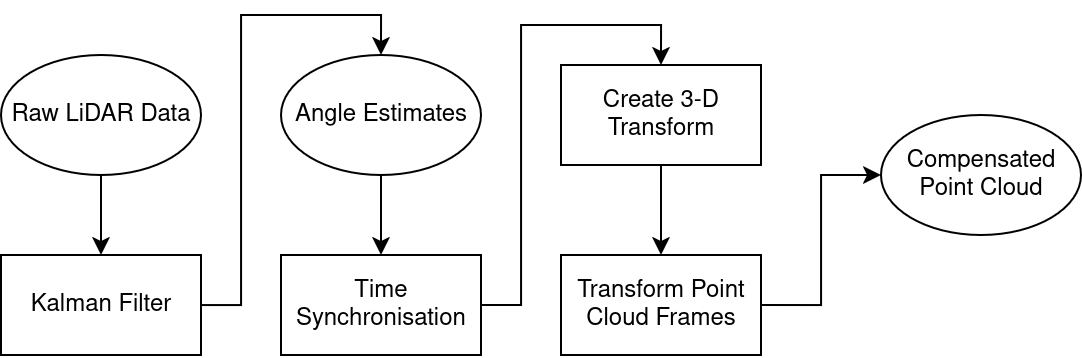
\includegraphics[width=0.82\textwidth]{figs/motion_comp.png}
    \caption{\textbf{Motion Compensation Pipeline}}
    \label{fig:motion_compensation}
\end{figure}
%----------------------------------------------------

Angle estimate residuals (the difference between the motion capture ground truth and the filter's estimates) were computed for the two test cases and used as the primary metric for comparing the filters relative performance. The residuals were also used in the tuning of both filters. To tune each filter's parameters, iterative adjustments were made to the parameters, and the angle estimates observed until the mean residuals reached a minimum, as recommended by \cite{grewalApplicationsKalmanFiltering2010}.
 

%====================================================
\section{De-noising}
\label{sec:ch6.section3}
%----------------------------------------------------

The return intensity of points can be used to remove or ignore unwanted points. A simple threshold filtering function can be constructed for de-noising data collected under snowy or other adverse conditions. To prevent valid points in the target scene with low return intensities from being discarded, a distance parameter was included in the threshold function.

*this needs to be redone*

%----------------------------------------------------
\begin{figure}[H]
    \centering
    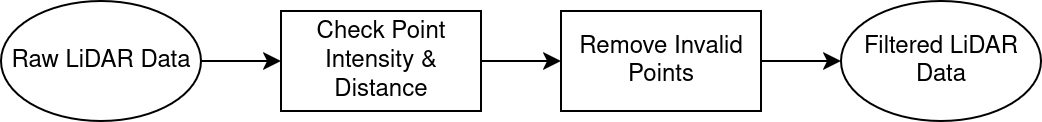
\includegraphics[width=0.8\textwidth]{figs/threshold_pipe.png}
    \caption{\textbf{De-noising Pipeline}}
    \label{fig:threshold_pipe}
\end{figure}
%----------------------------------------------------

The return intensity threshold was set to 1 and the distance threshold to 15 m. These values were selected to remove the maximum amount of noise points while minimizing the number of valid points removed.

%====================================================
\section{Wave Parameter Estimation}
\label{sec:ch6.section4}
%----------------------------------------------------

The Aalto University wave and ice tank probe data can be used as ground truth for wave parameter estimates. Wave models were fitted to the two datasets (wave probe and Avia) and magnitude and period estimates derived from the Avia data were compared to those from the wave probe.

As there was no time synchronisation between the Avia and wave probe, instantaneous wave parameters could not be compared. Instead, overall wave parameters (amplitude and frequency) for the duration of the tests were modelled and compared. 

The strict constraints on the wave behaviours allows for the wave models used to be greatly simplified. It can be assumed the waves will propagate uniformly across the tank with minimal change in direction and velocity.

Using the MATLAB \emph{curveFitter} tool, a sinusoidal model (equation \ref{eqn:probe_sin}) of wave height over time was fitted to the Aalto wave probe data from each test, producing a single amplitude and period value per test.

%----------------------------------------------------
\begin{equation} \label{eqn:probe_sin}
    y = Asin(\omega t + c)
\end{equation}
%----------------------------------------------------

\textit{y} is the wave height at time \textit{t}, \textit{A} is  amplitude, \textit{$\omega$} is the  angular frequency and \textit{c} is the phase shift. For this investigation, only amplitude and angular frequency (\textit{A} and \textit{$\omega$}) are of interest.

*talk more about how RANSAC was built*

To model the waves from point cloud data, a spatial sinusoidal plane model (equation \ref{eqn:avia_sin}) was fitted to each frame in the point cloud using \ac{RANSAC}. Each frame fit was run for 300 iterations at an inlier tolerance of 0.02 m (2 cm).

%----------------------------------------------------
\begin{equation} \label{eqn:avia_sin}
    z = Asin(Bx + C) + Dx + Ey + F
\end{equation}
%----------------------------------------------------

\textit{x}, \textit{y} and \textit{z} are co-ordinates of the wave relative to the Avia's origin. \textit{A} is the amplitude, \textit{B} is the wave number, \textit{C} is the phase shift and \textit{D} and \textit{E} are plane slopes and \textit{F} is an offset. For this investigation only amplitude and wave number (\textit{A} and \textit{B}) are of interest.

As the waves generated in the wave tank were waves in deep water, (water depth greater than half the wavelength), wave number (\textit{k}) is related to angular velocity (\textit{$\omega$}) through the dispersion relation (\cite{dingemansWaterWavePropagation1997}) given in equation \ref{eqn:dispersion}.

%----------------------------------------------------
\begin{equation} \label{eqn:dispersion}
    \omega = \sqrt{gk}
\end{equation}
%----------------------------------------------------

Wave angular velocity (\textit{$\omega$}) can be converted to period (\textit{T}) by the relation given in equation \ref{eqn:period}.

%----------------------------------------------------
\begin{equation} \label{eqn:period}
    T = \frac{2\pi}{\omega} 
\end{equation}
%----------------------------------------------------

Once all estimations were converted to wave period, the mean period and amplitude for each test, as determined by the Avia data were computed for comparison against the wave probe ground truth data.

%----------------------------------------------------
\begin{figure}[H]
    \centering
    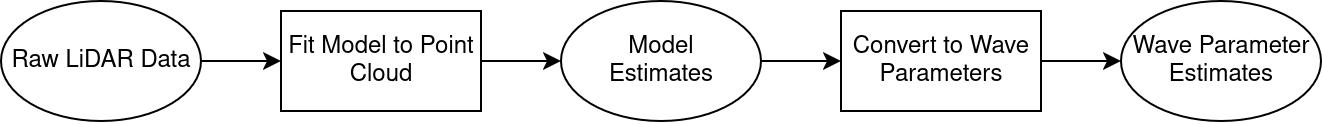
\includegraphics[width=\textwidth]{figs/wave_est.png}
    \caption{\textbf{Wave Parameter Estimation Pipeline}}
    \label{fig:wave_est}
\end{figure}
%----------------------------------------------------

%====================================================
\section{Pancake Identification}
\label{sec:ch6.section5}
%----------------------------------------------------

To identify the shape and size of individual pancakes in the point cloud data, three density-based clustering algorithms were investigated; \ac{DBScan}, \ac{VDBScan} and \ac{OPTICS}. 

Each of these algorithms accept a point cloud frame as input and return a list, where each entry in the list corresponds to a point in the input point cloud frame. Each entry contains a cluster identification number, indicating which cluster the point belongs to. Points that are classified as noise or outliers are given a cluster ID of -1. This list can then be used to visualise the clusters by assigning each cluster a unique colour, or to calculate the size and shape of individual pancakes by grouping points with the same cluster ID. 

As no ground truth data was available for pancake size and shape, the performance of each clustering algorithm was evaluated qualitatively by visual inspection of the clustering results and comparing the number of points assigned to each cluster.

To tune the parameters of each algorithm, multiple clustering runs were performed on the same point cloud frame with different parameter combinations. The results of each run were visually inspected and compared to determine which parameter combination produced the best clustering result (most coherent pancake shapes with least over- or under-inclusion of points).

%----------------------------------------------------
\subsection{DBScan}
\label{subsec:ch6.section5.subsec1}

The \ac{DBScan} algorithm was implemented using MATLAB's built-in \emph{dbscan} function, and is an unmodified version of the original algorithm.

%----------------------------------------------------
\subsection{VDBScan}
\label{subsec:ch6.section5.subsec2}

The \ac{VDBScan} algorithm implemented was adapted from MATLAB’s \emph{dbscan} function, with modifications to incorporate variable-density clustering as described by \cite{liuVDBSCANVariedDensity2007}. In contrast to the original \ac{VDBScan} approach, which assigns an individual \textbf{$\epsilon$} value to each point, this implementation estimates a set of candidate \textbf{$\epsilon$} values for the entire point cloud using the selected \textbf{k}-nearest neighbour distances. Traditional \ac{DBScan} clustering is then applied iteratively for each \textbf{$\epsilon$} value. The resulting cluster assignments from all runs are combined on a point-by-point basis, where the most frequently occurring cluster ID across all \textbf{$\epsilon$} values is chosen as the final label for that point.

The decision to use a modified \ac{VDBScan} implementation was made due to computational restraints. The original \ac{VDBScan} algorithm requires the calculation and storage of an individual \textbf{$\epsilon$} value for each point in the point cloud, which requires significant memory resources for large point clouds. Every attempt to run the original \ac{VDBScan} algorithm on the PC used for this investigation (equipped with 32 GB of RAM) resulted in out-of-memory errors. 

%----------------------------------------------------
\subsection{OPTICS}
\label{subsec:ch6.section5.subsec3}

The \ac{OPTICS} algorithm used was provided by \cite{daszykowskiMatlabCodeOPTICS2002}, and is an implementation with minor modifications for use in MATLAB.

%****************************************************
% END
%****************************************************